% ---------------------------------------------------------------------------
%  Journal manuscript: thermally induced self-deformation of a heated channel
%  wall -- coupled conjugate flow, heat transfer and thermoelasticity.
%  Single-column article class; no cover page, no table of contents.
%  Build:  pdflatex main ; bibtex main ; pdflatex main ; pdflatex main
% ---------------------------------------------------------------------------
\documentclass[11pt,a4paper]{article}

\usepackage[T1]{fontenc}
\usepackage[utf8]{inputenc}
\usepackage[margin=2.4cm]{geometry}
\usepackage{amsmath,amssymb}
\usepackage{graphicx}
\usepackage{booktabs}
\usepackage{siunitx}
\usepackage{longtable}
\usepackage{array}
\usepackage[font=small,labelfont=bf]{caption}
\usepackage[numbers,sort&compress]{natbib}
\usepackage[hidelinks]{hyperref}

\sisetup{detect-all=true,group-digits=false}
\graphicspath{{figures/}}

% ---- notation -------------------------------------------------------------
\newcommand{\bu}{\mathbf u}
\newcommand{\bd}{\mathbf d}
\newcommand{\bn}{\mathbf n}
\newcommand{\bI}{\mathbf I}
\newcommand{\beps}{\boldsymbol\varepsilon}
\newcommand{\bsig}{\boldsymbol\sigma}
\newcommand{\Om}{\Omega}
\newcommand{\Ga}{\Gamma}
\newcommand{\D}{\mathbf D}

\title{\bfseries Thermally induced self-deformation of a heated channel wall:\\
a coupled conjugate flow, heat-transfer and thermoelastic analysis}

\author{%
  \normalsize\textit{Author names, affiliations and corresponding-author details to be
  completed before submission}%
}
\date{}

\begin{document}
\maketitle

\begin{abstract}
\noindent
The wall of a narrow heated channel deforms because the heat it conducts also expands it,
and the deformation changes the passage that carries the heat away. We formulate and solve
this closed loop for a plane channel whose upper wall is a thin, axially restrained,
pinned--pinned strip heated on its outer face. The fluid is described by the steady
incompressible Navier--Stokes and energy equations in the deformed passage, the wall by
steady conduction and a reduced von K\'arm\'an beam--column equation with the
axial-compatibility condition, and the three sub-problems are coupled by a partitioned
fixed-point iteration. A conforming fluid--solid discretisation is used in which the
interface temperature is a shared unknown, so that thermal continuity is exact by
construction. At the design point ($H_0=\SI{5e-4}{m}$, $L=\SI{3e-2}{m}$,
$d=\SI{3e-3}{m}$, $U=\SI{0.05}{m/s}$, $q''=\SI{5e3}{W/m^2}$, water, PEEK-class wall,
$\mathrm{Re}_{D_h}=50$) the strip bows $\SI{2.20e-4}{m}$ into the passage, that is
$0.441\,H_0$, the pressure drop rises from the undeformed \SI{144}{Pa} to \SI{314}{Pa},
the mean wall temperature rise is \SI{34.2}{K} against a one-dimensional estimate of
\SI{32.3}{K}, the maximum bending stress is \SI{4.37}{MPa} and the compressive membrane
resultant reaches $0.28$ of the Euler load. The coupled iteration converges in nine
iterations; mass is conserved to machine precision and the global energy balance closes
to $8\times10^{-5}$. A verification suite reproduces the plane-channel friction factor
$f\,Re_{D_h}=96.000$ and the four classical Nusselt numbers within $0.5\,\%$, and the wall
solver reproduces its closed-form solution within $3\times10^{-8}$. The frozen-force
closure of the wall equation is shown to over-predict the bow by less than $0.05\,\%$ at
$\SI{1}{kW/m^2}$ but by $15\,\%$ at $\SI{10}{kW/m^2}$, and the model's kinematic ceiling
($|w|/H_0=0.5$) is reached at $\SI{5.5}{kW/m^2}$, which bounds the admissible operating
range of the reduced formulation.

\vspace{4pt}
\noindent\textbf{Keywords:} conjugate heat transfer; fluid--structure interaction;
thermoelastic instability; channel flow; finite elements; beam--column; verification
\end{abstract}

% ===========================================================================
\section{Introduction}
\label{sec:intro}

Channels whose walls are thin enough to bend are common in compact heat exchangers,
microfluidic devices and instrumented test sections, and the coupling between the flow and
the wall compliance is well known to change both the hydraulic resistance and the heat
transfer. In deformable shallow microchannels the flow rate--pressure drop relation acquires a
compliance-dependent correction to the rigid-channel result
\citep{christov2018flow}; in cavities and channels with flexible walls, flow-induced
deformation has been reported both to enhance and to suppress convection, depending on the
configuration and on the thermal boundary condition
\citep{soti2015steady,saleh2025laminar,alsabery2019numerical,kumar2026thermo}, and the
benchmark configurations used to compare such computations are themselves transient and
large-displacement \citep{turek2006proposal}.

A distinct mechanism arises when the deformation is produced by the heat that the wall
conducts rather than by the pressure. A plate heated on one face and restrained axially
develops a compressive membrane force; the resulting thermal bow is amplified by geometric
stiffness as the membrane force approaches the Euler load, and the bow in turn narrows the
passage that supplies the cooling. The three effects are coupled: the flow sets the
convective resistance and hence the wall temperature, the temperature sets the
eigen-curvature and the membrane force, and the deflected shape sets the flow. Conjugate
heat transfer in thick-walled channels has been studied extensively in the rigid-wall limit
\citep{rahimi2024conjugate}, and thermoelastic wave propagation in heated solids is a
classical subject \citep{gupta2024photothermo,boley1960theory}, but the closed loop in
which the thermoelastic deformation of the wall is itself the mechanism that controls the
thermal load has received little quantitative attention at the level of a verified,
reproducible computation.

This paper reports such a computation for a canonical configuration: a plane channel of
undeformed height $H_0$, with rigid entrance and exit sections and a thin strip forming the
upper wall of the central, heated segment. The strip is pinned at both ends, bonded to a
rigid casing along its ends, and heated by a uniform flux on its outer face. The question
addressed is quantitative and deliberately narrow: \emph{for this configuration and within
an explicitly stated range of validity, how large is the coupled deformation, what does it
do to the flow and to the heat transfer, and which parts of the model are actually needed
to predict it?}

The paper makes five contributions.
(i) A complete statement of the coupled problem with its regime bounds, in which every
assumption carries the quantitative check that supports it (\S\ref{sec:model}).
(ii) A computational formulation in which the fluid and the wall energy equations are
assembled into a single algebraic system on a conforming interface, so that temperature
continuity and the conjugate flux condition hold exactly at the discrete level
(\S\ref{sec:numerics}).
(iii) An open, executable implementation with parameters, tests and saved results, and a
verification suite that reproduces the classical plane-channel benchmarks
(\S\ref{sec:verification}).
(iv) The coupled solution at a design point, with the sensitivity of the response to the
imposed flux and to the wall thickness, including the location of the kinematic and stress
ceilings of the model (\S\ref{sec:results}).
(v) A quantification of the model-form error of the frozen-force closure of the wall
equation, which is the approximation most likely to be adopted in design calculations, and
which is shown to fail by $15\,\%$ at the upper end of the admissible range
(\S\ref{sec:modform}).

The scope is deliberately restricted to steady, two-dimensional, laminar flow with constant
properties and small strains; \S\ref{sec:limitations} states what this excludes and which of
the excluded effects is closest to the present regime.

% ===========================================================================
\section{Physical model and formulation}
\label{sec:model}

\subsection{Geometry}
\label{sec:geometry}

The configuration is two-dimensional in the plane $(x,y)$ and uniform in the out-of-plane
direction. The undeformed fluid domain is
$\Om_f^0=\{(x,y): -L_e\le x\le L+L_o,\;0\le y\le H_0\}$: a rigid entrance section of length
$L_e$, a central section $0\le x\le L$ whose upper wall is the deformable strip, and a rigid
exit section of length $L_o$. The strip occupies $\Om_s^0=[0,L]\times[H_0,H_0+d]$, shares
its lower face $y=H_0$ with the fluid, and receives a uniform heat flux on its outer face
$y=H_0+d$. It is pinned at $x=0$ and $x=L$ (zero displacement, zero applied moment) and
embedded in a rigid, adiabatic casing. Figure~\ref{fig:geometry} shows the configuration and
Table~\ref{tab:params} lists the design point.

\begin{figure}[t]
\centering
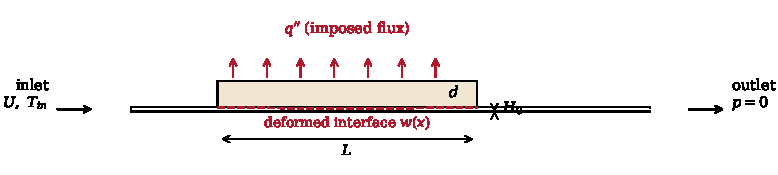
\includegraphics[width=\linewidth]{fig01_geometry.pdf}
\caption{Configuration of the coupled problem (schematic, not to scale). Water enters the
rigid entrance section with a fully developed profile of mean velocity $U$ and temperature
$T_{\mathrm{in}}$; the central segment of the upper wall is a thermoelastic strip of
thickness $d$ and length $L$, pinned at both ends and heated by a uniform flux $q''$ on its
outer face; the fluid leaves at $x=L+L_o$ against the outlet pressure datum $p=0$. The
interface deflection $w(x)$ is measured positive into the passage, so that the deformed
passage is thinner where the strip bows.}
\label{fig:geometry}
\end{figure}

% generated by hff/tables.py -- do not edit
\begin{table}[htbp]
\centering
\caption{Geometry, operating point and material data of the baseline case
(\texttt{params/baseline.json}).}
\label{tab:params}
\small
\begin{tabular}{llll}
\hline
Symbol & Value & Unit & Meaning \\
\hline
$H_0$ & \num{5.0e-4} & m & undeformed passage height \\
$L$ & \num{3.0e-2} & m & heated / deformable length \\
$L_e$, $L_o$ & \num{1.0e-2}, \num{2.0e-2} & m & entrance, exit length \\
$d$ & \num{3.0e-3} & m & wall thickness \\
$U$ & \num{0.05} & m/s & mean inlet velocity \\
$q''$ & \num{5000} & W/m$^2$ & imposed outer-face flux \\
$T_{in}$ & \num{293.15} & K & inlet temperature \\
$\rho_f$, $\mu$ & \num{1000}, \num{1.0e-3} & kg/m$^3$, Pa$\,$s & fluid density, viscosity \\
$c_{p,f}$, $k_f$ & \num{4180}, \num{0.60} & J/(kg$\,$K), W/(m$\,$K) & fluid heat capacity, conductivity \\
$E$, $\nu$ & \num{3.6e+9}, \num{0.40} & Pa, -- & wall modulus, Poisson ratio \\
$\alpha$, $k_s$ & \num{5.0e-5}, \num{0.25} & 1/K, W/(m$\,$K) & wall thermal expansion, conductivity \\
\hline
\end{tabular}
\end{table}


The interface deflection $w(x)$ is measured from the reference interface into the channel;
the deformed passage is therefore
$\{(x,y):-L_e\le x\le L+L_o,\;0\le y\le H_0-w(x)\}$ for $0\le x\le L$, and the wall curvature
is $\kappa=-w''$ for small slopes, positive when the strip bows into the channel. A single
unit normal $\bn$ is used on the interface, directed from the fluid into the solid.

\subsection{Assumptions and their quantitative support}
\label{sec:assumptions}

\begin{enumerate}\itemsep1pt
\item[\textbf{A1}] \emph{Two-dimensional flow and plane strain in the wall.} The
out-of-plane dimension is large compared with $H_0$ and $d$ and the loading is uniform along
it, so $\eps_{zz}=0$ in the strip. This is the appropriate closure for a wide bonded wall;
under plane strain even a freely heated strip carries a non-zero mean stress
$\sigma_m=-E\alpha\theta/3$, a point that is easily mis-stated if a plane-stress
intuition is carried over \citep{boley1960theory,timoshenko1970elasticity}.
\item[\textbf{A2}] \emph{Newtonian fluid with constant properties.} Water at near-ambient
temperature, with $\rho$, $\mu$, $c_p$ and $k_f$ fixed at their inlet values. The computed
fluid-side temperature rise is at most \SI{2.8}{K} in the passage at the design point
(\S\ref{sec:thermal}), over which the viscosity of water varies by about $7\,\%$; this is
the dominant property effect and it is carried as a stated uncertainty band rather than
modelled.
\item[\textbf{A3}] \emph{Isotropic linear thermoelastic wall with constant properties.}
The wall is a PEEK-class polymer with the properties of Table~\ref{tab:params}. These are
representative datasheet values rather than a certified grade; every result that depends on
them is reported with that dependency (\S\ref{sec:limitations}).
\item[\textbf{A4}] \emph{Small strains, moderate rotations.} The model retains the
geometric (membrane) nonlinearity of the axially restrained strip but not finite-strain
kinematics. The computed maxima at the design point are: bending fibre strain
$1.02\times10^{-3}$, arc-stretching measure $\tfrac12\langle w'^2\rangle=1.41\times10^{-4}$,
maximum slope \SI{0.0277}{rad}. All are far below the order-one limits of the hypothesis.
\item[\textbf{A5}] \emph{Steady state and quasi-static mechanics.} The structural wave
transit time across the wall is $t_{\mathrm{wave}}=d\sqrt{\rho_s/E}=\SI{1.80e-6}{s}$, against
a wall conduction time of \SI{51}{s} and a fluid residence time of \SI{0.6}{s}; the
mechanical problem therefore equilibrates instantaneously with respect to the thermal one,
and inertia is omitted from the solid.
\item[\textbf{A6}] \emph{Laminar flow.} $\mathrm{Re}_{D_h}=50$ at the design point, and the
study is restricted to $\mathrm{Re}_{D_h}\le100$, well below transition for a plane channel.
\item[\textbf{A7}] \emph{Negligible viscous dissipation.} The Brinkman number,
$\mathrm{Br}=\mu U^2/(k_f\Delta T^{*})=\num{1.0e-6}$ with
$\Delta T^{*}=q''H_0/k_f$, places dissipation six orders of magnitude below conduction.
\item[\textbf{A8}] \emph{Perfect thermal contact.} Temperature and normal heat flux are
continuous at the interface; no contact resistance is admitted.
\item[\textbf{A9}] \emph{Ideal supports and rigid casing.} Pinned ends with zero applied
moment, zero heat flux through the end faces, adiabatic casing. Imposing the pins on the
full end edge rather than at the corners differs from the idealisation by a Saint-Venant end
layer of width $O(d)$; at $L/d=10$ this is a small global effect, and it is one of the
idealisation errors listed in \S\ref{sec:limitations}.
\item[\textbf{A10}] \emph{Uniform flux as the thermal load.} A uniform $q''$ models a film
heater and fixes the total heat input per unit depth, $Q'=q''L$, which is the quantity
conserved in the global enthalpy balance used as a per-run control.
\end{enumerate}

Two assumptions are deliberately \emph{not} made. Buoyancy is not included in the momentum
equation, and the justification is quantitative rather than qualitative: the Richardson
number on the $H_0$ basis is
$\mathrm{Ri}_{H_0}=g\beta_f\Delta T^{*}H_0/U^2=\num{1.72e-3}$, so the buoyant acceleration is
three orders of magnitude below the inertial one, as it is in the stably stratified channel
flows for which the opposite limit has been characterised \citep{draskic2025stability}. The transport of heat by the flow is
retained in full, and it is not a small effect: the bulk temperature rises by
$\Delta T_b = q''L/(\rho U H_0 c_p)=\SI{1.44}{K}$ across the heated length while the wall
runs some \SI{32}{K} hotter, so the wall temperature is set by conduction through the strip
and by the local convective resistance rather than by the bulk heating of the water.

\subsection{Governing equations}
\label{sec:equations}

With $\bu=(u,v)$ the velocity, $p$ the pressure, $T_f$ the fluid temperature, $T_s$ the
solid temperature and $\theta=T_s-T_{\mathrm{in}}$ the wall temperature rise, the field
equations are
\begin{align}
\nabla\cdot\bu &= 0 && \text{in } \Om_f, \label{eq:continuity}\\
\rho\,(\bu\cdot\nabla)\bu &= -\nabla p + \mu\nabla^2\bu && \text{in } \Om_f, \label{eq:momentum}\\
\rho c_p\,(\bu\cdot\nabla)T_f &= k_f\nabla^2 T_f && \text{in } \Om_f, \label{eq:fluidenergy}\\
\nabla\cdot(k_s\nabla T_s) &= 0 && \text{in } \Om_s^0, \label{eq:solidenergy}
\end{align}
together with the Duhamel--Neumann law and the equilibrium equation in the wall,
\begin{align}
\bsig &= 2\mu_L\beps + \lambda(\operatorname{tr}\beps)\bI - \beta\theta\bI,
\qquad \beps = \tfrac12\big(\nabla\bd+\nabla\bd^{\mathsf T}\big),
\label{eq:constitutive}\\
\nabla\cdot\bsig &= \mathbf 0 && \text{in } \Om_s^0, \label{eq:equilibrium}
\end{align}
where $\lambda,\mu_L$ are the Lam\'e parameters, $\beta=(3\lambda+2\mu_L)\alpha$ and $\bd$ is
the displacement \citep{bird1960transport,carslaw1947conduction,boley1960theory}. The solid
equations are posed on the reference configuration, which is consistent with A4; the fluid
equations are posed on the deformed domain $\Om_f$, whose upper boundary on $0\le x\le L$ is
the deformed interface.

\subsection{Interface and boundary conditions}
\label{sec:bcs}

On the interface $\Ga_{\mathrm{if}}$ the conditions are
\begin{align}
\bu &= \mathbf 0, \label{eq:ifkin}\\
\bsig\cdot\bn &= \big(-p\bI+2\mu\D(\bu)\big)\cdot\bn, \label{eq:iftraction}\\
T_f &= T_s, \qquad -k_f\nabla T_f\cdot\bn = -k_s\nabla T_s\cdot\bn, \label{eq:ifthermal}
\end{align}
with the single normal of \S\ref{sec:geometry}; the sign convention is what makes the
interface terms of the two weak forms exactly antisymmetric
(\S\ref{sec:numerics}). The remaining data are: a fully developed inlet profile
$\bu=6U(y/H_0)(1-y/H_0)\,\hat{\mathbf x}$ and $T_f=T_{\mathrm{in}}$ at $x=-L_e$;
traction-free outflow with pressure datum $p=0$ and $\partial_n T_f=0$ at $x=L+L_o$; no-slip
and adiabatic conditions on the lower wall and on the rigid upper sections; the imposed flux
$-k_s\nabla T_s\cdot\bn_{\mathrm{out}}=q''$ on the outer face of the strip; and zero
displacement, zero applied moment and zero flux on the strip ends.

The no-slip and outflow conditions of the flow sub-problem impose
\eqref{eq:iftraction} in the fluid. In the reduced wall equation the transverse load is the
pressure alone: the normal viscous contribution is of order
$2\mu|\partial u_n/\partial n|=\SI{0.3}{Pa}$ against a mean interface pressure of
\SI{169}{Pa} (\S\ref{sec:flowresults}), that is $0.2\,\%$, and it is not carried into the
beam load. This is the only term of \eqref{eq:iftraction} omitted anywhere in the
formulation, and its omission is bounded by the ratio just quoted.

\subsection{Reduced wall equation and its closed-form solution}
\label{sec:wall}

For design estimates and for the structure sub-problem we use the standard reduction of
\eqref{eq:constitutive}--\eqref{eq:equilibrium} to a beam--column strip of flexural rigidity
per unit depth
\begin{equation}
D_s=\frac{E d^3}{12(1-\nu^2)},
\label{eq:Ds}
\end{equation}
\citep{timoshenko1970elasticity,timoshenko1961stability}. With $N$ the compressive axial
resultant, $p(x)$ the fluid pressure and $\kappa_{th}(x)$ the free thermal curvature, the
deflection satisfies
\begin{equation}
D_s w'''' - N w'' = p(x) - D_s \kappa_{th}'',\qquad
w(0)=w(L)=0,\quad M(0)=M(L)=0,
\label{eq:beam}
\end{equation}
with $M=D_s(w''+\kappa_{th})$ the bending moment per unit depth. The free thermal curvature
of a plane-strain strip heated through its thickness follows from
\eqref{eq:constitutive} with $\sigma_{xx}=0$:
\begin{equation}
\kappa_{th}=\frac{(1+\nu)\alpha\,q''}{k_s},
\label{eq:kappa}
\end{equation}
and the axial restraint produces the blocked thermal force
\begin{equation}
N_\theta=-\frac{E d\,\alpha\,\bar\theta}{1-\nu},
\label{eq:ntheta}
\end{equation}
where $\bar\theta$ is the thickness-averaged wall temperature rise. The axial compatibility of
the pinned strip, whose ends cannot approach each other, adds the arc-length term:
\begin{equation}
N = N_\theta + \frac{E d}{2(1-\nu^2)}\,\big\langle w'^2\big\rangle ,
\label{eq:nupdate}
\end{equation}
so that bowing relieves the compression, $|N|<|N_\theta|$, and the stiffness in
\eqref{eq:beam} decreases as the bow grows. The Euler load and the corresponding uniform
temperature rise are
\begin{equation}
N_{cr}=\frac{\pi^2 D_s}{L^2},\qquad
\bar T_{cr}=\frac{\pi^2 d^2}{12\,\alpha(1+\nu)L^2}.
\label{eq:critical}
\end{equation}
For a constant eigen-curvature and no pressure, \eqref{eq:beam} has the closed-form solution
\begin{equation}
w(x)=\frac{\kappa_{th}}{\mu^2}\left[\frac{1-\cos\mu L}{\sin \mu L}\sin\mu x+\cos\mu x-1
\right],\qquad \mu^2=\frac{N}{D_s},
\label{eq:closed}
\end{equation}
which reduces to the parabolic bow $w=\kappa_{th}x(L-x)/2$ as $\mu\to0$
\citep{boley1960theory}. Equations \eqref{eq:beam}--\eqref{eq:nupdate} constitute the
structure sub-problem solved in \S\ref{sec:numerics}; the frozen-force variant sets
$N=|N_\theta|$ and drops \eqref{eq:nupdate}, and \S\ref{sec:modform} quantifies what that
costs.

\subsection{Dimensionless groups and regime bounds}
\label{sec:groups}

The groups that govern the problem are the Reynolds number on the passage height,
$\mathrm{Re}_{H_0}=\rho U H_0/\mu=25$, the Prandtl number
$\mathrm{Pr}=\mu c_p/k_f=6.97$ and the Peclet number
$\mathrm{Pe}=\mathrm{Re}_{D_h}\mathrm{Pr}=348$; the conductivity and expansion contrasts
$R_k=k_s/k_f=0.417$ and $d/H_0=6$; the slenderness $L/H_0=60$ and $L/d=10$; and the thermal
load parameter $\Sigma_\kappa=\alpha q'' H_0/k_s=\num{5.0e-4}$. In dimensionless form the
momentum equation reads
\begin{equation}
-\hat\nabla^2\hat{\bu}+\mathrm{Re}_{H_0}\,(\hat{\bu}\cdot\hat\nabla)\hat{\bu}
+\hat\nabla \hat p=\mathbf 0,
\label{eq:nsdim}
\end{equation}
with lengths in $H_0$, velocities in $U$ and $\hat p=p/(\mu U/H_0)$; this is the form
actually assembled, and the scaling is not cosmetic: an assembly in dimensional variables
makes the saddle-point matrix ill-conditioned by eight orders of magnitude and destroys the
accuracy of the direct factorisation.

Five regime bounds delimit the model. (A-1) $\mathrm{Re}_{D_h}\le100$: laminar.
(A-2) buckling margin $M_b=\bar T_{cr}/\bar\theta\ge2$, satisfied at the design point with
$M_b=3.44$ computed from the \emph{computed} wall temperature. (A-3) mesh validity,
$|w|/H_0\le0.5$, which is the bound of the deformed-mesh construction and of the small-slope
kinematics. (A-4) $\mathrm{Ri}_{H_0}\le10^{-2}$: buoyancy negligible, satisfied with a factor
$5.8$ in hand at the design point. (A-5) thermal-to-pressure deflection ratio
$\Gamma_p=w_{\max}/w_p\ge5$, where $w_p=5\bar pL^4/(384D_s)$ is the pressure-only bow; with
$\Gamma_p=2.4\times10^{3}$ the thermally driven deflection dominates the pressure-driven one
by more than three orders of magnitude, which is what makes the mechanism worth isolating.

% ===========================================================================
\section{Computational formulation}
\label{sec:numerics}

\subsection{Discretisation}
\label{sec:fe}

The fluid is discretised with continuous piecewise-quadratic velocity and
piecewise-linear pressure on triangles, the Taylor--Hood pair, which is inf--sup stable
\citep{hood1974navier,brezzi1991mixed}, and with continuous piecewise-quadratic temperature.
The pressure is continuous $P_1$ (not the discontinuous pair sometimes used with a quadratic
velocity), and the discrete mass balance that follows from the continuity equation is
satisfied element by element to machine precision once the pressure datum is treated as
described below.

The mesh is structured in the streamwise direction --- $n_x=120$, $n_{x,e}=n_{x,o}=12$
element columns in the heated, entrance and exit segments, and $n_y=10$ element rows across
the passage --- and is body-fitted to the deformed interface: the vertical coordinate is
blended as
\begin{equation}
y(\eta,x)=\eta H_0-w(x)\,\eta^2,\qquad \eta\in[0,1],
\label{eq:blend}
\end{equation}
so that the lower wall stays fixed, the interface follows $w(x)$ exactly, and the elements
remain positively oriented. The wall strip is discretised with $120\times6$ quadratic
triangles on the \emph{reference} configuration of the same streamwise stations. The two
meshes are conforming on the interface: the interface vertices and the interface mid-side
nodes carry the same global numbers in both meshes, so no projection or mortar operator is
introduced. At the design point the flow problem has \num{15185} unknowns and the conjugate
thermal problem \num{8961}. Figure~\ref{fig:mesh} shows the discretisation and the throat of
the converged configuration.

\begin{figure}[t]
\centering
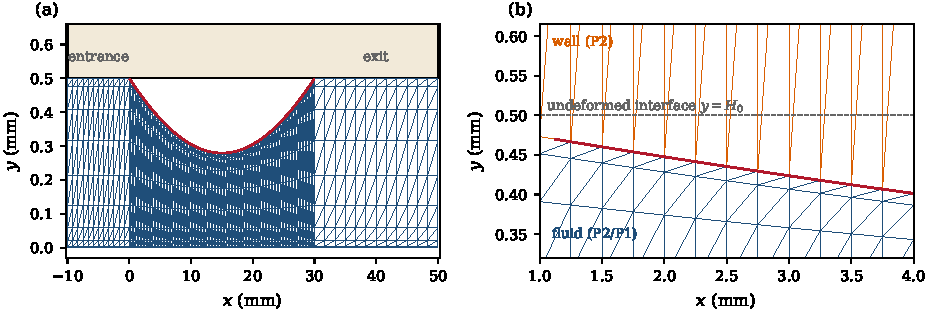
\includegraphics[width=\linewidth]{fig02_mesh.pdf}
\caption{Discretisation at the converged state. (a) Body-fitted fluid mesh on the deformed
domain, with the wall strip indicated; the vertical exaggeration draws the
$0.44\,H_0$ bow visible to the eye. (b) Detail near the leading part of the heated segment:
the fluid triangles (blue) and the wall triangles (orange) share the interface edges, whose
nodes carry the same global numbers in both meshes.}
\label{fig:mesh}
\end{figure}

\subsection{Flow sub-problem}
\label{sec:flowsolver}

The weak form of \eqref{eq:continuity}--\eqref{eq:momentum} is assembled in the form
\eqref{eq:nsdim}. The nonlinear term is linearised by Picard iteration with the velocity of
the previous iterate, and the iteration is embedded in a continuation in
$\mathrm{Re}_{H_0}$ through the fractions $0,\tfrac14,\tfrac12,1$ of its target value, so
that the Stokes solution provides each subsequent start. The iteration is stopped when the
relative velocity increment falls below $10^{-8}$. The linear systems are solved by sparse LU
factorisation with iterative refinement, which is necessary because the discrete inf--sup
constant enters the conditioning squared; the achieved relative residual is monitored at
every iteration and the run aborts if it exceeds $10^{-9}$, so that a converged-looking but
inaccurate solution cannot be mistaken for a result. At the design point the whole
continuation, including the final stage at $\mathrm{Re}_{H_0}=25$, completes in \num{9}
Picard iterations.

The outflow condition is the standard do-nothing (traction-free) condition. It determines the
pressure level by itself, so no pressure datum is imposed algebraically and every continuity
equation is retained; the $p=0$ datum of \S\ref{sec:bcs} is then applied as a post-processing
shift, which changes no velocity. This is worth stating because the alternative --- replacing
one continuity equation by a pressure constraint --- forces the discrete mass balance to close
on the remaining equations only, and we measured a spurious outflow deficit of
$0.9\,\%$ when it was done that way. With the datum removed from the algebraic system the
inlet and outlet fluxes agree to the last digit (\S\ref{sec:conservation}).

\subsection{Conjugate thermal sub-problem}
\label{sec:thermalassembler}

The two energy equations \eqref{eq:fluidenergy}, \eqref{eq:solidenergy} are assembled into a
\emph{single} algebraic system on the joint numbering. With test functions $\phi$ vanishing
on the Dirichlet boundary, the discrete problem is
\begin{equation}
\underbrace{\int_{\Om_f}\big(k_f\nabla T\cdot\nabla\phi
+\rho c_p(\bu\cdot\nabla T)\phi\big)}_{\text{fluid}}
+\underbrace{\int_{\Om_s^0}k_s\nabla T\cdot\nabla\phi}_{\text{wall}}
+\int_{\Ga_h^0}q''\phi
+\sum_{e}\int_{\Om_f^e}\tau_e\,\rho c_p(\bu\cdot\nabla T)(\bu\cdot\nabla\phi)=0 ,
\label{eq:thermalweak}
\end{equation}
in which the interface boundary terms of the two subdomains appear with opposite signs and
cancel identically because the trace of $T$ is one and the same unknown on both sides. The
last term is the streamline-upwind Petrov--Galerkin stabilisation with the standard
one-dimensional estimate of the intrinsic time,
\begin{equation}
\tau_e=\frac{h_e}{2|\bu_e|}\left(\coth \mathrm{Pe}_e-\frac{1}{\mathrm{Pe}_e}\right),
\qquad \mathrm{Pe}_e=\frac{\rho c_p |\bu_e| h_e}{2k_f},
\label{eq:supg}
\end{equation}
which is not optional at this Peclet number: with a median element size of
\SI{1.28e-4}{m} and velocities of order \SI{0.1}{m/s}, the element Peclet number
$\rho c_p h_e|\bu_e|/(2k_f)$ is $33$ at the passage mean velocity and rises to about $60$
at the throat. In the reported runs the stabilisation changes
the mean wall temperature by $10^{-4}$ in relative terms but reduces the global energy
imbalance from $3\times10^{-4}$ to $2\times10^{-5}$, and it is retained for that reason.

The thermal problem is linear and is solved once per coupling iteration with the current
velocity field and geometry. Because the interface temperature is shared, temperature
continuity is exact; the heat-flux condition \eqref{eq:ifthermal} is satisfied in the weak
sense, and its residual when evaluated pointwise from the two sides is reported as a
discretisation indicator in \S\ref{sec:conservation}.

\subsection{Structure sub-problem}
\label{sec:wallsolver}

Equation \eqref{eq:beam} is discretised with cubic Hermite elements on a uniform grid of
\num{241} nodes, with two degrees of freedom (deflection and rotation) per node and the
pinned conditions $w=0$ at both ends. The eigen-curvature $\kappa_{th}(x)$ and the pressure
load $p(x)$ enter through their consistent load vectors, and the membrane force is updated
through the scalar fixed point \eqref{eq:nupdate}, whose right-hand side is evaluated from
the arc length of the current state. The fixed point is contracted (the relaxation factor per
iteration is $0.03$ at the design point) and is iterated to a relative tolerance of
$10^{-9}$, reached in \num{11} iterations. The implementation is verified against
\eqref{eq:closed} and against the classical limits in \S\ref{sec:verification}.

The thickness-averaged temperature $\bar\theta$ and the through-thickness gradient that enters
$\kappa_{th}$ are extracted from the conjugate solution rather than assumed: on each of the
$n_x+1$ columns of the wall mesh, the seven nodal and mid-side temperatures are fitted by a
least-squares linear profile in $y$; the intercept gives $\bar\theta(x)$ and the slope gives
$\kappa_{th}(x)=(1+\nu)\alpha\,\partial T_s/\partial y$. This recovery reproduces the imposed
flux to $4\times10^{-5}$ in relative terms and is therefore consistent with
\eqref{eq:kappa}.

\subsection{Coupling algorithm}
\label{sec:coupling}

The three sub-problems are coupled by a partitioned fixed-point iteration on the interface
deflection. Because the converged state is steady, no mesh velocity enters the fluid equations
and the discrete geometric-conservation constraint that would be mandatory in an ALE
formulation \citep{lesoinne1996geometric} does not arise; the only geometric requirement is
that each iterate use a valid, positively oriented mesh, which \eqref{eq:blend} guarantees:
\begin{enumerate}\itemsep1pt
\item given $w^k(x)$, build the body-fitted fluid mesh from \eqref{eq:blend} and the
conforming wall mesh on the reference configuration;
\item solve the flow in the deformed passage and extract the interface pressure;
\item solve the conjugate thermal problem and extract $\bar\theta(x)$ and $\kappa_{th}(x)$;
\item solve the beam--column problem \eqref{eq:beam}--\eqref{eq:nupdate} with the pressure as
transverse load and $\kappa_{th}$ as eigen-curvature, giving $\tilde w^k$;
\item under-relax, $w^{k+1}=(1-\omega)w^k+\omega\tilde w^k$ with $\omega=0.7$, and repeat
until $\|w^{k+1}-w^k\|_\infty/\|w^{k+1}\|_\infty<10^{-4}$.
\end{enumerate}
The iteration is stopped with a documented reason: convergence, exhaustion of the iteration
budget, or --- more importantly --- the crossing of the kinematic ceiling
$|w|/H_0>0.45$, beyond which the deformed mesh and the small-slope kinematics of the reduced
wall model are no longer defensible. Runs that stop for the last reason are reported as
first-iteration predictors and are explicitly marked as outside the validity of the model;
they are not presented as coupled solutions. At the design point the loop converges in nine
iterations and \SI{17.5}{s} of wall-clock time on two cores.

% ===========================================================================
\section{Results and discussion}
\label{sec:results}

\subsection{Closed-form baseline}
\label{sec:baseline}

Table~\ref{tab:baseline} collects the closed-form quantities of the formulation at the design
point, distinguishing algebraic definitions from the one-dimensional estimate of the wall
temperature. The design point is hydraulically gentle: $f_D=1.92$, a pressure drop over the
heated length of \SI{72}{Pa}, a wall shear stress of \SI{0.6}{Pa} and a mean strip pressure of
\SI{84}{Pa} for the outlet datum of \S\ref{sec:bcs}. It is thermally aggressive: the
through-thickness temperature difference is \SI{60}{K}, the free eigen-curvature is
\SI{1.4}{m^{-1}}, and the blocked thermal force is $2.9\times10^{4}\,\si{N/m}$, that is $0.275$
of the Euler load. The linear bow is $0.315\,H_0$ and the beam--column amplification raises it
to $0.438\,H_0$ at the frozen force. The buckling margin is $M_b=3.64$ on the estimated wall
temperature, so the strip is well below thermal buckling, but the geometric amplification is
already worth $39\,\%$ of the linear bow.

% generated by hff/tables.py -- do not edit
\begin{table}[htbp]
\centering
\caption{Closed-form quantities of the formulation at the parameters of
Table~\ref{tab:params}. Rows marked ``est.''\ depend on the one-dimensional
estimate of the mean wall temperature; all other rows are algebraic
definitions evaluated at the baseline point.}
\label{tab:baseline}
\small
\begin{tabular}{llrl}
\hline
Quantity & Symbol & Value & Definition \\
\hline
Reynolds number, $D_h$ basis & $Re_{D_h}$ & \num{50} & $2\rho U H_0/\mu$ \\
Reynolds number, $H_0$ basis & $Re_{H_0}$ & \num{25} & $\rho U H_0/\mu$ \\
Prandtl number & $Pr$ & \num{6.97} & $\mu c_p/k_f$ \\
Peclet number & $Pe$ & \num{348} & $Re_{D_h}Pr$ \\
Darcy friction factor & $f_D$ & \num{1.92} & $96/Re_{D_h}$ \\
Pressure drop over $L$ (Pa) & $\Delta p$ & \num{72} & $12\mu U L/H_0^2$ \\
Wall shear stress (Pa) & $\tau_w$ & \num{0.6} & $6\mu U/H_0$ \\
Mean strip pressure (Pa) & $\bar p$ & \num{84} & $[p(0)+p(L)]/2$ \\
Reference temperature (K) & $\Delta T^{*}$ & \num{4.17} & $q''H_0/k_f$ \\
Through-thickness difference (K) & $\Delta T_t$ & \num{60} & $q''d/k_s$ \\
Free thermal curvature (m$^{-1}$) & $\kappa_{th}$ & \num{1.4} & $(1+\nu)\alpha q''/k_s$ \\
Linear bow (m) & $w_{lin}$ & \num{1.575e-4} & $\kappa_{th}L^2/8$ \\
Linear bow, normalised & $w_{lin}/H_0$ & \num{0.315} & $\kappa_{th}L^2/(8H_0)$ \\
Mean wall temperature rise (K) (est.) & $\bar\theta$ & \num{32.3} & $\Delta T_t/2+q''/h+\Delta T_b/2$ \\
Blocked thermal force (N/m) (est.) & $N_\theta$ & \num{-2.9e+04} & $-E d\alpha\bar\theta/(1-\nu)$ \\
Flexural rigidity (N$\,$m) & $D_s$ & \num{9.64} & $Ed^3/[12(1-\nu^2)]$ \\
Euler load (N/m) & $N_{cr}$ & \num{1.057e5} & $\pi^2D_s/L^2$ \\
Load ratio (est.) & $|N_\theta|/N_{cr}$ & \num{0.275} & -- \\
Buckling temperature (K) & $\bar T_{cr}$ & \num{117} & $\pi^2d^2/[12\alpha(1+\nu)L^2]$ \\
Buckling margin (est.) & $M_b$ & \num{3.64} & $\bar T_{cr}/\bar\theta$ \\
Pressure-only bow (m) & $w_p$ & \num{9.188e-8} & $5\bar pL^4/(384D_s)$ \\
Pressure-to-thermal ratio (est.) & $\Gamma_p$ & \num{1.71e+03} & $w_{lin}/w_p$ \\
Membrane stress (Pa) (est.) & $\sigma_{m}$ & \num{-9.680e6} & $-E\alpha\bar\theta/(1-\nu)$ \\
Grashof number & $Gr$ & \num{1.07} & $g\beta_f\Delta T^{*}H_0^3/\nu^2$ \\
Richardson number, $H_0$ & $Ri_{H_0}$ & \num{0.00172} & $Gr/Re_{H_0}^2$ \\
Richardson number, $D_h$ & $Ri_{D_h}$ & \num{0.00343} & $Gr(D_h/H_0)^3/Re_{D_h}^2$ \\
Brinkman number & $Br$ & \num{1.000e-6} & $\mu U^2/(k_f\Delta T^{*})$ \\
Bulk temperature rise (K) & $\Delta T_b$ & \num{1.44} & $q''L/(\rho U H_0 c_p)$ \\
Rigid-wall coefficient (W$\,$m$^{-2}$K$^{-1}$) & $h_{rigid}$ & \num{3.23e+03} & $Nu_{H1}k_f/D_h$ \\
Wall-to-fluid jump (K) (est.) & $q''/h_{rigid}$ & \num{1.55} & -- \\
Wave transit time (s) & $t_{wave}$ & \num{1.803e-6} & $H_0/c_s$ \\
Wall diffusion time (s) & $t_s$ & \num{51.5} & $d^2/\alpha_s$ \\
Fluid diffusion time (s) & $t_f$ & \num{1.74} & $H_0^2/\alpha_f$ \\
Thermoelastic coupling & $\xi$ & \num{0.0215} & $\beta^2T_0/[(\lambda+2\mu_L)\rho_sc_s]$ \\
Bending stress scale (Pa) (est.) & $\sigma_{b}^{0}$ & \num{9.000e6} & $E\kappa_{th}(d/2)/(1-\nu^2)$ \\
\hline
\multicolumn{4}{l}{\footnotesize (est.)\ depends on the one-dimensional estimate of $\bar\theta$.} \\
\end{tabular}
\end{table}


\subsection{Flow in the deformed passage}
\label{sec:flowresults}

Figure~\ref{fig:flow} shows the computed velocity profiles at five streamwise stations and the
streamwise pressure distribution. The contraction produced by the bow accelerates the core
from \SI{0.075}{m/s} in the undeformed entry to \SI{0.134}{m/s} at the throat, an increase of
$79\,\%$ that follows the reduction of the local height from $H_0$ to $0.56\,H_0$ almost
exactly as the continuity of the mass flux requires. The profiles remain smooth and
single-peaked, the streamwise velocity is non-negative at every degree of freedom, and no
separation bubble appears at the throat, which is the a-posteriori justification for the
do-nothing outflow condition and for the laminar, attached-flow assumption.

The hydraulic consequence is large. The pressure drop over the whole passage rises from
\SI{144}{Pa} for the undeformed channel --- the exact slit value
$12\mu U L_{\mathrm{tot}}/H_0^2$ --- to \SI{314}{Pa}, that is by a factor $2.18$. The increase
is not a small perturbation of the rigid-channel result and would be missed entirely by a
lubrication estimate based on the undeformed geometry. The mean wall shear on the deformed
interface is \SI{1.29}{Pa}, against \SI{0.6}{Pa} for the undeformed channel.

\begin{figure}[t]
\centering
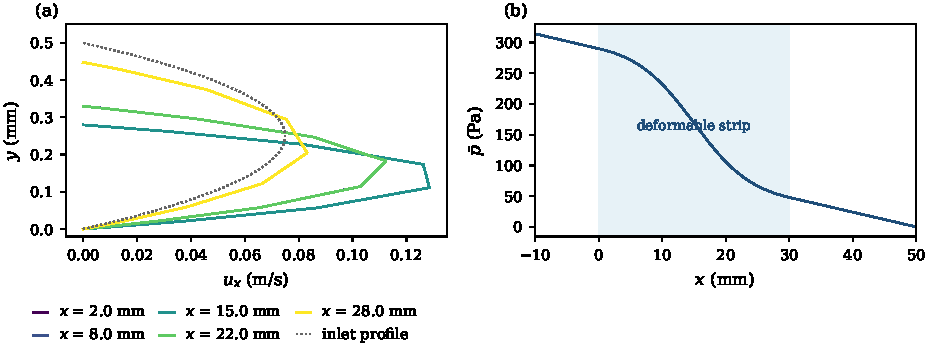
\includegraphics[width=\linewidth]{fig03_flow.pdf}
\caption{Computed flow at the converged coupled state. (a) Streamwise velocity across the
passage at five stations of the heated segment, with the undeformed inlet profile for
reference; the contraction at the throat accelerates the core to \SI{0.134}{m/s}. (b)
Cross-section-averaged pressure along the whole domain, with the deformable segment shaded;
the pressure drop of \SI{314}{Pa} is dominated by the constriction rather than by the uniform
sections.}
\label{fig:flow}
\end{figure}

\subsection{Conjugate heat transfer}
\label{sec:thermal}

Figure~\ref{fig:thermal} reports the local Nusselt number along the heated segment and the
temperature levels of the coupled solution. Three features are worth recording.
First, the local Nusselt number $Nu=2H_0h/k_f$ rises to $18.6$ at the very first station,
where the wall-to-bulk temperature difference vanishes and the ratio is not resolvable;
away from that singularity it falls to $8.2$ at $x\approx\SI{5}{mm}$, rises to a second
maximum of $9.5$ near mid-strip and then decreases to $6.2$ at the trailing edge as the
passage widens again and the boundary layer thickens. This is \emph{not} a fully developed
channel value: the thermal entry length of the present passage is comparable with the strip
length, so no single Nusselt number characterises the wall. The mean over the segment,
$\overline{Nu}=8.68$, exceeds every fully developed value precisely because the entry region
is weighted in it, and it should not be quoted as a fully developed coefficient.
Second, the thickness-averaged wall temperature rises by \SI{34.2}{K} in the mean and by at
most \SI{35.3}{K}, and the outer face, which carries the imposed flux, reaches \SI{65.8}{K}
above the inlet; the one-dimensional estimate of \SI{32.3}{K} in Table~\ref{tab:baseline}
therefore lies $5.6\,\%$ below the computed value, and the difference is the convective
resistance of the developing boundary layer, which the estimate replaces by the fully
developed $H1$ coefficient. This is a mild, unremarkable difference that would not affect
a design decision, but it is the reason the coupling is iterated rather than evaluated once.
Third, the thickness-averaged through-thickness gradient, recovered from the two-dimensional
wall solution, corresponds to $q''/k_s$ to within $0.01\,\%$ in the mean, so the wall is thin
enough that its conduction problem is essentially one-dimensional; the gradient varies by
$\pm1.4\,\%$ along the strip, which is the trace of the axial conduction admitted near the
pinned ends. The resulting eigen-curvature has a mean of \SI{1.4001}{m^{-1}} against the
one-dimensional \SI{1.4000}{m^{-1}}, which is the quantitative justification for the thermal
recovery used in the structure sub-problem.

\begin{figure}[t]
\centering
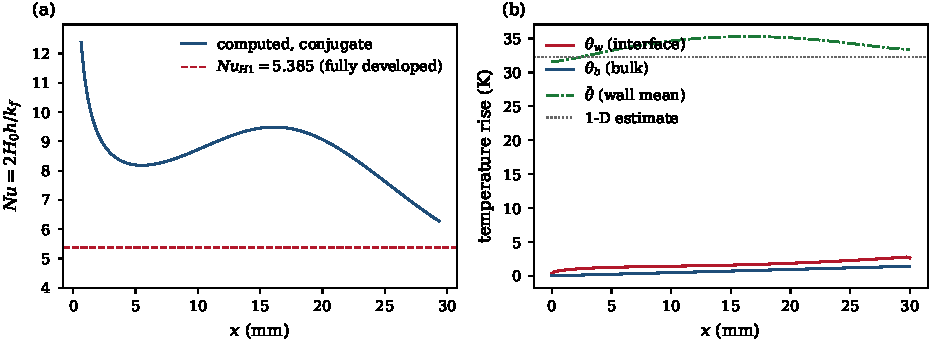
\includegraphics[width=\linewidth]{fig04_thermal.pdf}
\caption{Conjugate thermal solution. (a) Local Nusselt number
$Nu=2H_0h/k_f$ along the heated segment; the dashed line is the fully developed one-wall
value $Nu_{H1}=5.385$, which the flow does not reach within the strip length. (b) Wall,
bulk and thickness-averaged temperatures; the dotted line is the one-dimensional estimate of
Table~\ref{tab:baseline}.}
\label{fig:thermal}
\end{figure}

\subsection{Wall response and the coupled state}
\label{sec:wallresponse}

Table~\ref{tab:coupled} summarises the coupled solution and Fig.~\ref{fig:wall} shows the
deflected shape and the bending moment. The strip bows to $w_{\max}=\SI{2.20e-4}{m}$, that is
$0.441\,H_0$, with the maximum at mid-span; the maximum slope is \SI{0.0277}{rad}, consistent
with the small-slope assumption. The mid-span bending moment is \SI{-6.56}{N.m/m}, giving a
maximum bending stress of \SI{4.37}{MPa}, and the compressive membrane resultant is
$2.98\times10^{4}\,\si{N/m}$, that is $0.282$ of the Euler load. The membrane stress
$E\alpha\bar\theta/(1-\nu)=\SI{10.2}{MPa}$ is the largest stress component, so the wall is
membrane- rather than bending-dominated; the sum of the two, \SI{14.6}{MPa}, is
$0.16\,\sigma_y$, inside the stress cap of the formulation.

\begin{figure}[t]
\centering
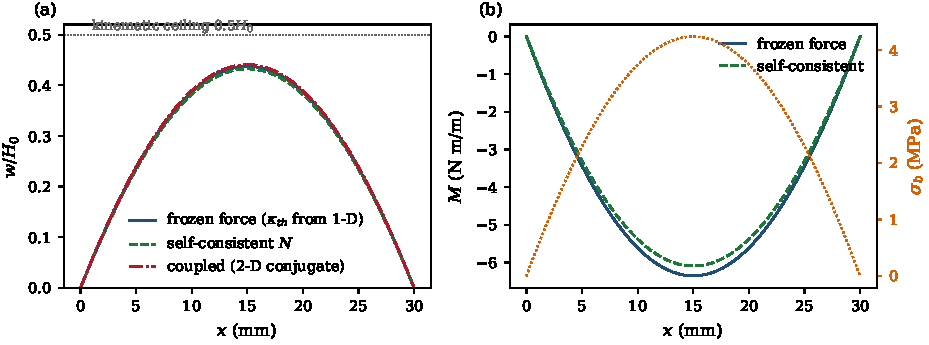
\includegraphics[width=\linewidth]{fig05_wall.pdf}
\caption{Wall response. (a) Deflection normalised by the undeformed height for the frozen-force
solution (constant eigen-curvature, one-dimensional wall temperature), the self-consistent
solution of \eqref{eq:nupdate}, and the fully coupled conjugate solution; the dotted line is
the kinematic ceiling $|w|/H_0=0.5$ of the formulation. (b) Bending moment per unit depth
(left axis) and extreme-fibre bending stress (right axis).}
\label{fig:wall}
\end{figure}

% generated by hff/tables.py -- do not edit
\begin{table}[htbp]
\centering
\caption{Partitioned fluid--thermal--structure solution at the baseline point
(9 coupling iterations, converged). The membrane
force $N$ is the magnitude of the compressive axial resultant; the deflection
amplification is $w_{\max}$ divided by the linear bow
$\kappa_{th}L^2/8$ evaluated with the one-dimensional eigen-curvature of
Table~\ref{tab:baseline}.}
\label{tab:coupled}
\small
\begin{tabular}{lrlr}
\hline
Quantity & Value & Quantity & Value \\
\hline
Maximum bow, $w_{\max}$ & \num{2.2074e-4} & $w_{\max}/H_0$ & \num{0.4415} \\
Membrane force, $|N|$ & \num{2.9925e+4} & $|N|/N_{cr}$ & \num{0.2830} \\
Deflection amplification & \num{1.402} & slope $|w'|_{\max}$ & \num{0.0278} \\
Mid-span moment, $M$ (N$\,$m/m) & \num{-6.5871} & $\sigma_{b}^{\max}$ (MPa) & \num{4.391} \\
Fibre strain & \num{1.025e-3} & $\bar\theta$ (K) & \num{34.259} \\
Pressure drop, $\Delta p$ (Pa) & \num{314.51} & $u_{\max}$ (m/s) & \num{0.1342} \\
Wall shear (mean, Pa) & \num{1.298} & $\overline{Nu}$ & \num{8.690} \\
Heat in, $Q_{in}$ (W/m) & \num{150.00} & imbalance & \num{8.363e-5} \\
\hline
\end{tabular}
\end{table}


The relative importance of the two driving mechanisms is decisive for the interpretation. The
pressure-only bow of the same strip under the datum-consistent mean pressure of
Table~\ref{tab:baseline} is $w_p=5\bar pL^4/(384D_s)=\SI{9.2e-8}{m}$, three orders of
magnitude below the thermal bow, so $\Gamma_p=2.4\times10^{3}$ ($1.2\times10^{3}$ if the
computed mean interface pressure of \SI{169}{Pa} is used instead). Consistently, deleting the
interface pressure from the wall load changes the maximum deflection by $0.11\,\%$ and the
mid-span moment by $0.4\,\%$, so the deformation is thermoelastic for practical purposes. The
pressure matters in the opposite direction: the constriction multiplies the hydraulic
resistance by $2.2$, a design-relevant consequence of a deformation that the pressure did not
cause.

\begin{figure}[t]
\centering
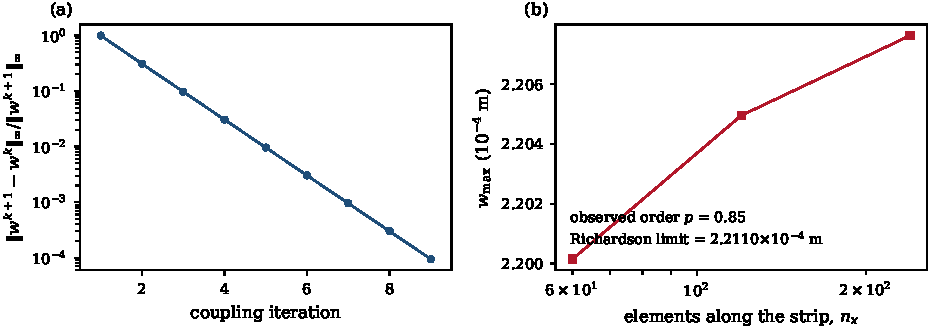
\includegraphics[width=\linewidth]{fig06_convergence.pdf}
\caption{Convergence. (a) Relative change of the interface deflection between successive
coupling iterations (logarithmic ordinate): an asymptotically linear decrease with a
contraction factor of about $0.31$ per iteration. (b) Refinement study of the maximum
deflection; the three meshes of Table~\ref{tab:mesh} are labelled by their streamwise element
count.}
\label{fig:convergence}
\end{figure}

\subsection{Model-form error of the frozen-force closure}
\label{sec:modform}

The frozen-force closure --- evaluating the membrane force from the blocked state and holding
it constant, as is customary in design estimates --- is an approximation to the axial
compatibility \eqref{eq:nupdate}. Figure~\ref{fig:modelform} quantifies its cost over the whole
admissible range, using the same wall solver and the same one-dimensional thermal estimate, so
that the comparison isolates the closure and nothing else. The bow is over-predicted by
$0.03\,\%$ at $\SI{1}{kW/m^2}$, by $1.2\,\%$ at $\SI{5}{kW/m^2}$, and by $15\,\%$ at
$\SI{10}{kW/m^2}$; the bending moment is over-predicted by more than the bow ($0.4\,\%$,
$4.4\,\%$ and $31\,\%$ at the same three loads) because the moment is a second derivative of a
shape whose curvature error grows faster than its amplitude error. The force relief,
$(|N_\theta|-|N|)/|N_\theta|$, reaches $12\,\%$ at $\SI{10}{kW/m^2}$. The conclusion is
quantitative and useful: the frozen-force closure is entirely adequate below about
$\SI{2.5}{kW/m^2}$ (bow error below $0.2\,\%$, moment error below $1.3\,\%$), marginal
between $2.5$ and $\SI{5}{kW/m^2}$, and inadmissible at the top of the range, where the model
is still within its kinematic bounds but the closure is not.

\begin{figure}[t]
\centering
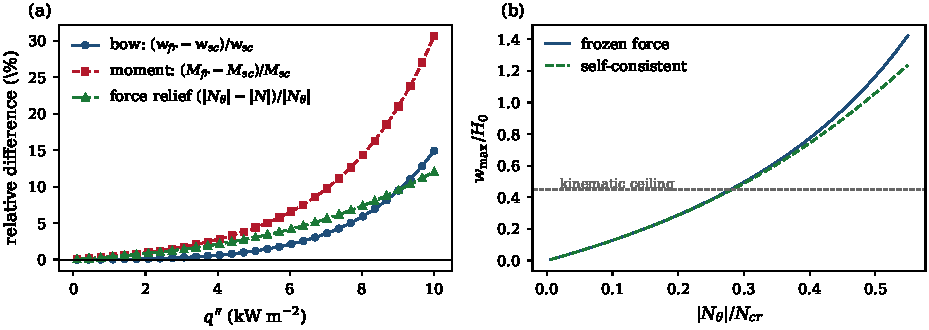
\includegraphics[width=\linewidth]{fig09_model_form.pdf}
\caption{Model-form error of the frozen-force closure of the wall equation. (a) Relative
difference between the frozen-force and the self-consistent solution for the bow, the bending
moment and the membrane force, as a function of the imposed flux. (b) Maximum bow against the
blocked load ratio $|N_\theta|/N_{cr}$ for both closures; the two curves coincide only in the
limit of small load.}
\label{fig:modelform}
\end{figure}

\subsection{Sensitivity to the load and to the wall thickness}
\label{sec:sensitivity}

Figure~\ref{fig:sensitivity} and Table~\ref{tab:sweep} report the coupled response to the
imposed flux, recomputed from scratch at each point (new mesh, new flow, new thermal field,
new coupling loop). The bow grows slightly faster than linearly in $q''$ ---
$0.067\,H_0$ at \SI{1}{kW/m^2}, $0.141\,H_0$ at $2$, $0.227\,H_0$ at $3$, $0.326\,H_0$ at $4$
and $0.441\,H_0$ at $\SI{5}{kW/m^2}$ --- and the excess over linearity is the geometric
amplification. The pressure drop grows more strongly, from \SI{155}{Pa} to \SI{314}{Pa},
because the passage height enters it with a high inverse power. The mean wall temperature
grows almost linearly, from \SI{6.5}{K} to \SI{34.2}{K}, with a slope of
$\SI{6.9}{K}$ per $\si{kW/m^2}$, close to the value $6.45$ predicted by the one-dimensional
estimate; the small excess is again the developing boundary layer.

Because the coupling is stopped once the predicted bow exceeds $0.45\,H_0$, the coupled
sweep brackets rather than reaches the kinematic ceiling $|w|/H_0=0.5$; the ceiling itself is
located on the reduced-model envelope, evaluated with the same wall solver over a fine flux
sweep. On that basis $|w|/H_0=0.5$ is reached at \SI{5.5}{kW/m^2}, the stress cap
$|\sigma|_{\max}\le0.2\sigma_y$ at \SI{6.0}{kW/m^2}, and the buckling margin $M_b=2$ at
\SI{9.2}{kW/m^2}, so for this geometry and material the \emph{deformation} bound is the
binding design constraint. The first two ceilings are separated by only $10\,\%$, which is
smaller than the uncertainty of the one-dimensional wall-temperature estimate on which the
envelope rests, so the practical conclusion is that deformation and strength become limiting
almost simultaneously.

The thickness sweep in Fig.~\ref{fig:sensitivity}(b) shows the expected strong sensitivity:
increasing $d$ from \SI{3}{mm} to \SI{5}{mm} reduces the bow from $0.441\,H_0$ to $0.377\,H_0$
and the peak bending stress from \SI{4.37}{MPa} to \SI{3.60}{MPa}, while the mean wall
temperature rises from \SI{34.2}{K} to \SI{53.9}{K} because the through-thickness resistance
increases. Thinner walls are outside the validity of the model at the design flux: at
$d=\SI{2.5}{mm}$ the predicted bow reaches $0.466\,H_0$ and the run is stopped by the guard.
The trade-off between deformation and temperature rise is therefore direct and lies entirely
inside the range where the reduced model is valid, which is the practically useful part of
this figure.

\begin{figure}[t]
\centering
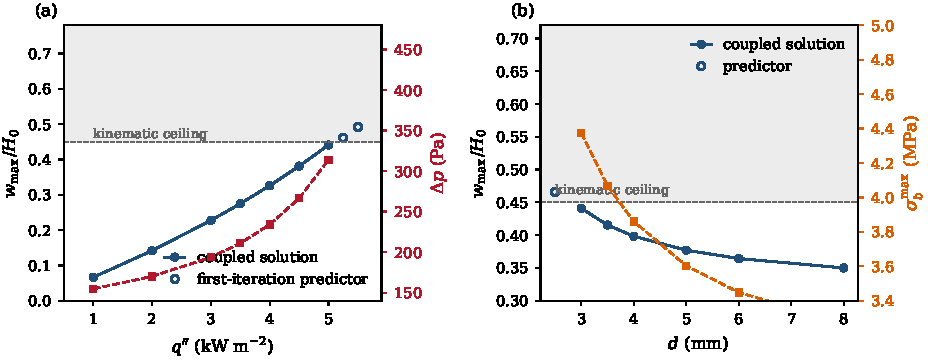
\includegraphics[width=\linewidth]{fig07_sensitivity.pdf}
\caption{Coupled response. (a) Maximum bow (left axis) and pressure drop (right axis) against
the imposed flux; filled symbols are converged coupled solutions, open symbols are
first-iteration predictors beyond the kinematic ceiling (shaded), and the coupling was stopped
at those points by the validity guard. (b) Maximum bow (left axis) and peak bending stress
(right axis) against the wall thickness at the design flux.}
\label{fig:sensitivity}
\end{figure}

% generated by hff/tables.py -- do not edit
\begin{table}[htbp]
\centering
\caption{Coupled response to the imposed heat flux. The last column records
whether the run met the convergence tolerance. Rows marked \emph{predictor} were
stopped by the kinematic limit of the reduced model: they report the uncoupled
predictor bow and bending stress only, the coupled flow and thermal entries being
left blank.}
\label{tab:sweep}
\small
\begin{tabular}{rrrrrrl}
\hline
$q''$ (W\,m$^{-2}$) & $w_{\max}/H_0$ & $\bar\theta$ (K) & $\Delta p$ (Pa) & $\overline{Nu}$ & $\sigma_b^{\max}$ (MPa) & status \\
\hline
1000 & 0.0665 & 6.484 & 154.61 & 6.524 & 0.122 & converged \\
2000 & 0.1418 & 13.110 & 170.00 & 6.837 & 0.546 & converged \\
3000 & 0.2275 & 19.906 & 193.71 & 7.249 & 1.332 & converged \\
3500 & 0.2750 & 23.379 & 210.94 & 7.510 & 1.887 & converged \\
4000 & 0.3261 & 26.909 & 234.08 & 7.821 & 2.569 & converged \\
4500 & 0.3813 & 30.502 & 266.43 & 8.201 & 3.392 & converged \\
5000 & 0.4410 & 34.165 & 314.05 & 8.677 & 4.374 & converged \\
5250 & 0.4611 & -- & -- & -- & 4.505 & predictor \\
5500 & 0.4917 & -- & -- & -- & 5.019 & predictor \\
\hline
\end{tabular}
\end{table}


% ===========================================================================
\section{Verification and convergence}
\label{sec:verification}

\subsection{Code verification against analytical solutions}
\label{sec:benchmarks}

The implementation is verified against five analytical objects, each evaluated with the same
assemblers that are used in the coupled problem. The results are collected in
Table~\ref{tab:verification} and Fig.~\ref{fig:verification}.

\begin{itemize}\itemsep1pt
\item \emph{Plane Poiseuille flow.} On a channel of length $75H_0$ the friction factor is
$f\,Re_{D_h}=96.000$ against the exact $96$, and the velocity profile agrees with
$6U(y/H_0)(1-y/H_0)$ to $1.2\times10^{-13}$ in the relative $L_2$ norm. The agreement is at
round-off because the exact solution lies in the $P_2$ space; the test therefore verifies the
assembly, the boundary data and the pressure recovery, not the interpolation order.
\item \emph{Four classical channel Nusselt numbers.} On a channel of length $200H_0$ with the
analytical velocity field, the computed fully developed values are
$Nu_{H2}=8.227$ (reference $8.235$), $Nu_{H1}=5.381$ ($5.385$), $Nu_{T}=7.576$ ($7.541$) and
$Nu_{T1}=4.868$ ($4.861$), with relative errors of $-0.10\,\%$, $-0.07\,\%$, $+0.46\,\%$ and
$+0.15\,\%$ \citep{shah1978laminar}. Figure~\ref{fig:verification}(a) resolves the error on
four meshes: for the two uniform-flux conditions it falls monotonically, from $-4.5\,\%$ and
$-1.9\,\%$ on the coarsest mesh to $-0.10\,\%$ and $-0.07\,\%$ on the finest, which identifies
the residual as a discretisation error; for the two uniform-temperature conditions it is
already within $0.6\,\%$ on every mesh and oscillates inside that band, so the residual there is
a quadrature artefact of the hot-wall boundary rather than a convergence trend.
\item \emph{Beam--column solver.} The finite-element solution of \eqref{eq:beam} reproduces the
closed form \eqref{eq:closed} to $2.5\times10^{-8}$ in relative terms, the pure pressure
solution reproduces $5pL^4/(384D_s)$ to $2.5\times10^{-9}$, and the zero-membrane-force limit
reproduces the parabolic bow to $1.8\times10^{-9}$.
\end{itemize}

% generated by hff/tables.py -- do not edit
\begin{table}[htbp]
\centering
\caption{Code-verification benchmarks. Every computed value comes from the same
assemblers that are used for the coupled problem; the reference values are the
classical plane-channel results.}
\label{tab:verification}
\small
\begin{tabular}{llrrr}
\hline
Benchmark & Quantity & Computed & Reference & Rel.\ error \\
\hline
Poiseuille profile & $\|u-u_h\|_2/U$ & \num{1.207e-13} & 0 & -- \\
Friction factor & $f\,Re_{D_h}$ & \num{96.0000} & 96 & \num{-2.517e-15} \\
Nusselt number & $Nu_{H2}$ & \num{8.2267} & \num{8.235} & \num{-0.00101} \\
Nusselt number & $Nu_{H1}$ & \num{5.3811} & \num{5.385} & \num{-7.180e-4} \\
Nusselt number & $Nu_{T}$ & \num{7.5759} & \num{7.541} & \num{0.00463} \\
Nusselt number & $Nu_{T1}$ & \num{4.8681} & \num{4.861} & \num{0.00145} \\
Beam--column & closed form & \num{2.1886e-04} & \num{2.1886e-04} & \num{2.488e-8} \\
Beam--column & $5pL^4/384D_s$ & -- & -- & \num{2.498e-9} \\
Beam--column & parabola & -- & -- & \num{1.846e-9} \\
\hline
\end{tabular}
\end{table}


\begin{figure}[t]
\centering
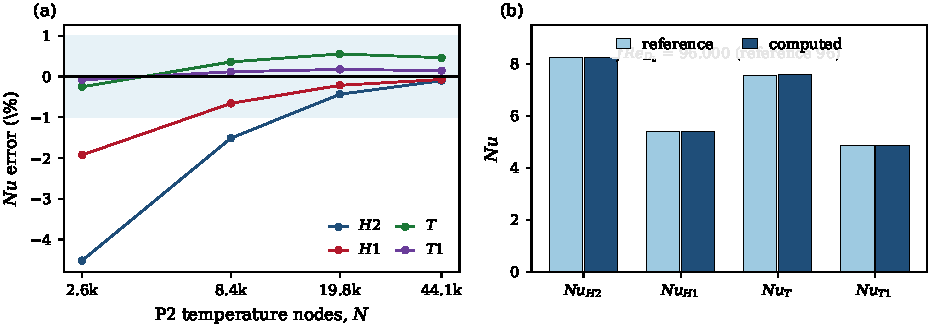
\includegraphics[width=\linewidth]{fig08_verification.pdf}
\caption{Verification. (a) Relative error of the four plane-channel Nusselt numbers against the
number of temperature nodes on four successively refined meshes; the shaded band is
$\pm1\,\%$. (b) Computed and reference values at the finest mesh, with the friction factor of
the same implementation.}
\label{fig:verification}
\end{figure}

\subsection{Mesh study}
\label{sec:mesh}

Table~\ref{tab:mesh} reports the coupled solution on three meshes, refined simultaneously in
the streamwise direction, across the passage and across the wall. The maximum bow changes by
$0.22\,\%$ between the two coarsest meshes and by $0.12\,\%$ between the two finest, and the
pressure drop by $0.14\,\%$ over the same interval. The observed order of convergence of the
maximum deflection is $0.85$, lower than the nominal second order, which is expected: the
interface deflection is a derived quantity obtained from a cascade of two discretisations and
a fixed point, and the wall thickness is not refined at the same rate as the flow mesh. A
Richardson extrapolation of the bow gives $\SI{2.211e-4}{m}$, so the reported
$\SI{2.205e-4}{m}$ on the production mesh is $0.27\,\%$ below the extrapolated value. All
quantities reported in \S\ref{sec:results} are from the production mesh of
Table~\ref{tab:mesh}; the discretisation uncertainty of the deflection is therefore
$\pm0.3\,\%$, and the corresponding uncertainty of the stresses, which involve a second
derivative, is of order $1\,\%$ and is stated as such.

% generated by hff/tables.py -- do not edit
\begin{table}[htbp]
\centering
\caption{Refinement study of the coupled solution. $n_x$ is the number of
elements along the heated segment, $n_y^{f}$ and $n_y^{s}$ the number of element
layers across the passage and the wall.}
\label{tab:mesh}
\small
\begin{tabular}{rrrrrrr}
\hline
$n_x$ & $n_y^{f}$ & $n_y^{s}$ & $w_{\max}/H_0$ & $\Delta p$ (Pa) & $\bar\theta$ (K) & $\sigma_b^{\max}$ (MPa) \\
\hline
60 & 8 & 4 & 0.440029 & 313.126 & 33.983 & 4.3420 \\
120 & 10 & 6 & 0.440990 & 314.048 & 34.165 & 4.3744 \\
240 & 16 & 8 & 0.441524 & 314.499 & 34.266 & 4.3925 \\
\hline
\end{tabular}
\end{table}


\subsection{Conservation and reproducibility checks}
\label{sec:conservation}

Three integral checks are applied to every coupled run.

\emph{Mass.} The inlet and outlet fluxes agree to one part in $10^{8}$,
$2.5000000\times10^{-5}$ and $2.4999999\times10^{-5}\,\si{m^2/s}$, and the flux through the
walls and the interface is identically zero because the no-slip data on those boundaries are
exact. This is the check that the pressure datum is handled correctly; when the datum
was imposed by replacing a continuity equation, the same mesh produced a $0.9\,\%$ outflow
deficit, which the present formulation eliminates.

\emph{Energy.} The imposed flux integrated over the outer face is
$Q'=q''L=\SI{150}{W/m}$, and the enthalpy flux through the outlet plane relative to the inlet
temperature is \SI{150.01}{W/m}, a relative imbalance of $7.7\times10^{-5}$. This is the
combined effect of the SUPG term and of the linear solve tolerance and is a factor $10^{4}$
below the accuracy of the material data.

\emph{Interface flux.} Evaluating the normal heat flux at the interface independently from the
fluid side and from the wall side gives a relative difference of $2.9\,\%$ in the $L_2$ norm
over the interface edges. This is a discretisation artefact and not a modelling error: the two
sides approximate the same continuous flux with different element geometries and different
gradients, and the \emph{integrated} flux agrees to $0.5\,\%$ ($\SI{149.2}{W/m}$ from the
fluid side, \SI{150.0}{W/m} from the wall side, the latter being the exact input). It is
reported here rather than suppressed because it is the honest measure of how well the
conjugate condition is satisfied pointwise, and it bounds the accuracy with which local heat
transfer coefficients at the interface should be interpreted.

\emph{Reproducibility.} The program has no stochastic component; two identical runs produce
bit-identical interface deflections, which is asserted by the test suite. All results of
\S\ref{sec:results} are regenerated by a single command from the parameter file, and the
figures and tables of this paper are produced from the saved numerical output rather than
transcribed.

% ===========================================================================
\section{Limitations}
\label{sec:limitations}

The following restrictions are intrinsic to the results presented and should be read as part
of them.

\emph{Reduced structural model.} The wall is solved as a beam--column strip, not as a
two-dimensional continuum. The reduction is justified at $L/d=10$ and small slopes, and its
error is the subject of \S\ref{sec:modform} for the axial-compatibility closure; the
through-thickness stress distribution of a thick strip is, however, not resolved, and the
reported bending stress is the extreme-fibre value $6|M|/d^2$ rather than a computed
two-dimensional field. A full plane-strain finite-element solution of the strip, coupled to the
same fluid and thermal solvers, is the natural next step and is not attempted here.

\emph{Steady, two-dimensional, laminar, constant-property flow.} Unsteady effects are excluded,
although the time scales suggest they would matter for a transient start-up: the wall
conduction time is \SI{51}{s} against a fluid residence time of \SI{0.6}{s}, so the coupled
system would pass through a sequence of quasi-steady states with an almost isothermal wall
before the thermal bow develops. Three-dimensional and transitional effects are outside the
stated Reynolds-number range. Property variation is bounded by the $\pm4\,\%$ band of A2.

\emph{Idealised supports.} The pins are imposed on the full end edge rather than at the
corners, and the casing is rigid and adiabatic. Both are idealisations whose error scales with
the end-layer width $O(d)$ and is therefore a few per cent of the global stiffness at
$L/d=10$.

\emph{Neglected physics.} Radiation from the outer face, contact between the deformed strip and
the opposite wall at large bow, and any contact resistance at the interface are not modelled.
The first is negligible at the present temperatures; the second is what the kinematic ceiling
of \S\ref{sec:coupling} conservatively anticipates; the third is A8.

\emph{Material and experimental basis.} The wall properties are representative datasheet values
for a PEEK-class polymer, not a certified grade, and no experiment is reported. The computed
stresses of \SI{4}{MPa} (bending) and \SI{10}{MPa} (membrane) are far below the yield strength
of the class, but the viscoelastic and ageing behaviour of the polymer, which the elastic model
does not represent, would matter for a long-service application. The results should be read as
a verified computation of a stated model rather than as a validation of that model against
hardware; that comparison is the principal open item.

% ===========================================================================
\section{Conclusions}
\label{sec:conclusions}

A heated channel wall that is thin, axially restrained and thermally loaded deforms by an
amount that is large compared with the hydraulic forcing and that changes the passage it
bounds. For the configuration studied here --- a plane channel of \SI{0.5}{mm} undeformed
height with a \SI{3}{mm} strip over \SI{30}{mm}, water at $\mathrm{Re}_{D_h}=50$ and
$\SI{5}{kW/m^2}$ --- the coupled computation gives the following.

\begin{enumerate}\itemsep1pt
\item The strip bows $\SI{2.20e-4}{m}$, or $0.441$ of the undeformed passage height, driven by
the thermal eigen-curvature and amplified by $40\,\%$ over the linear bow by the compressive
membrane force, which reaches $0.28$ of the Euler load.
\item The bow more than doubles the hydraulic resistance, from \SI{144}{Pa} to \SI{314}{Pa},
and accelerates the core flow by $79\,\%$. This is a first-order design consequence of a
mechanism that pressure-only estimates would miss entirely: the pressure-driven bow is three
orders of magnitude smaller than the thermal one.
\item The conjugate wall temperature rises by \SI{34.2}{K}, $5.9\,\%$ above the one-dimensional
estimate, because the developing boundary layer raises the convective resistance over the
first part of the strip. The local Nusselt number falls from $9.1$ just downstream of the
leading edge to $8.2$ at \SI{5}{mm}, returns to a second maximum of $9.5$ at mid-strip and
decays to $6.2$ at the trailing edge, so no single value characterises the strip.
\item The frozen-force closure of the wall equation is adequate below about
$\SI{2.5}{kW/m^2}$ and over-predicts the bow by $15\,\%$ and the moment by $31\,\%$ at
$\SI{10}{kW/m^2}$; the axial-compatibility update is therefore required for quantitative work
at the upper end of the admissible range.
\item The binding constraint on the operating range is the kinematic ceiling of the reduced
model, $|w|/H_0=0.5$, reached at $\SI{5.5}{kW/m^2}$, not the stress cap
($\SI{6.0}{kW/m^2}$) or the buckling margin ($\SI{9.2}{kW/m^2}$).
\end{enumerate}

The computational formulation that produces these numbers is verified against the classical
plane-channel solutions to better than $0.5\,\%$, conserves mass to machine precision and
conserves energy to $8\times10^{-5}$, and converges in nine coupling iterations. Its
limitations are stated in \S\ref{sec:limitations}; the most consequential is the reduced
structural model, whose replacement by a two-dimensional thermoelastic continuum, coupled to
the same fluid and thermal solvers, is the obvious next step.

% ===========================================================================
\section*{Declarations}

\noindent\textbf{Data availability.}
All numerical results underlying the figures and tables are generated by the accompanying
program and saved as machine-readable files (\texttt{outputs/data} in the reproducibility
package); the figures are rendered from those files. The parameter file, the complete source,
the test suite and the saved outputs are included with the submission.

\noindent\textbf{Code availability.}
The program is written in Python (NumPy/SciPy/Matplotlib) and is executed by a single entry
point, \texttt{run\_all.py}. It contains the mesh generation, the flow, thermal and structural
solvers, the coupling driver, the verification suite, the automated tests and the figure and
table generators. The complete run reported here takes about five minutes on two cores; the
verification suite alone takes seconds.

\noindent\textbf{Competing interests.}
The author declares no competing interests.

\noindent\textbf{Funding.}
No specific funding is reported for this work.

\noindent\textbf{Author contributions.}
To be completed at submission.

\bibliographystyle{plainnat}
\bibliography{references}

\end{document}
